\documentclass[11pt]{article}
\usepackage[margin=1in]{geometry}
\usepackage[dvipsnames]{xcolor}
\usepackage{graphicx,booktabs,amsmath,hyperref,caption,placeins}
\usepackage[T1]{fontenc}
\captionsetup{font=small,labelfont=bf}
\hypersetup{colorlinks=true,linkcolor=blue!50!black,urlcolor=blue!50!black}
\newcommand{\nmse}{\mathrm{nMSE}}

\title{Latent local fields for a CM1 squall line:\\ what the data say so far}
\author{Dalton Jones \and Claude}
\date{5 November 2026}

\begin{document}
\maketitle

\begin{abstract}
We asked whether the local latent field method of Papers~I--II carries over to a cloud model, using two-dimensional CM1 squall-line simulations. Three tests on the data alone come first. Information travels about 8--12\,km per 5-minute output frame, so a local model with a short stencil is viable. Five-minute output samples a roughly 10-minute cycle of the storm columns at about the Nyquist limit; 1-minute output resolves it. Forecast skill grows with the number of storms in the training set, not with the number of patches cut from them.

A learned model was then trained on CM1 ensembles that we generated. Each column is the vector of channels at one site, the boundaries are open, and the stencil propagator is trained with a forced halo. Trained on 28 one-minute members, it forecasts held-out members for an hour with error below the difference between two truth members, and holds the gust front within 0.8\,km for the first 20 minutes and 3.3\,km over the hour. Persistence drifts by nearly 12\,km over the same hour.
\end{abstract}

\section{Data}
The simulations are two-dimensional ($x$--$z$) squall lines from CM1 release 21.1:
\begin{itemize}
\item 400\,km by 20\,km, with 250\,m grid spacing in $x$ and 62 stretched levels;
\item open lateral boundaries, and a grid moving east at 12.5\,m\,s$^{-1}$;
\item Morrison two-moment microphysics, TKE turbulence, and no Coriolis force;
\item initialization by a 2\,K warm bubble in a Weisman--Klemp sounding.
\end{itemize}
The original set has 10 members at 5-minute output. They differ only by independent $\sim$0.1\,K perturbations to potential temperature below 500\,m. We rebuilt CM1 and generated \texttt{ens\_A} on CSU's Cashew cluster: 31 members with the same perturbation scheme, 6\,h each, at 1-minute output. All 31 members ran to completion, taking 72--93 minutes each on one core.

A model state is the column at each grid cell: $u'$, $w$, $\theta'$, $q_v'$ and $p'$ (deviations from the far-field initial column), and liquid and ice condensate as $\sqrt{q}$, over 62 levels. That is $7\times 62 = 434$ channels per cell. Figure~\ref{fig:sections} shows the storm and Figure~\ref{fig:hov} its evolution.

\begin{figure}[h]
\centering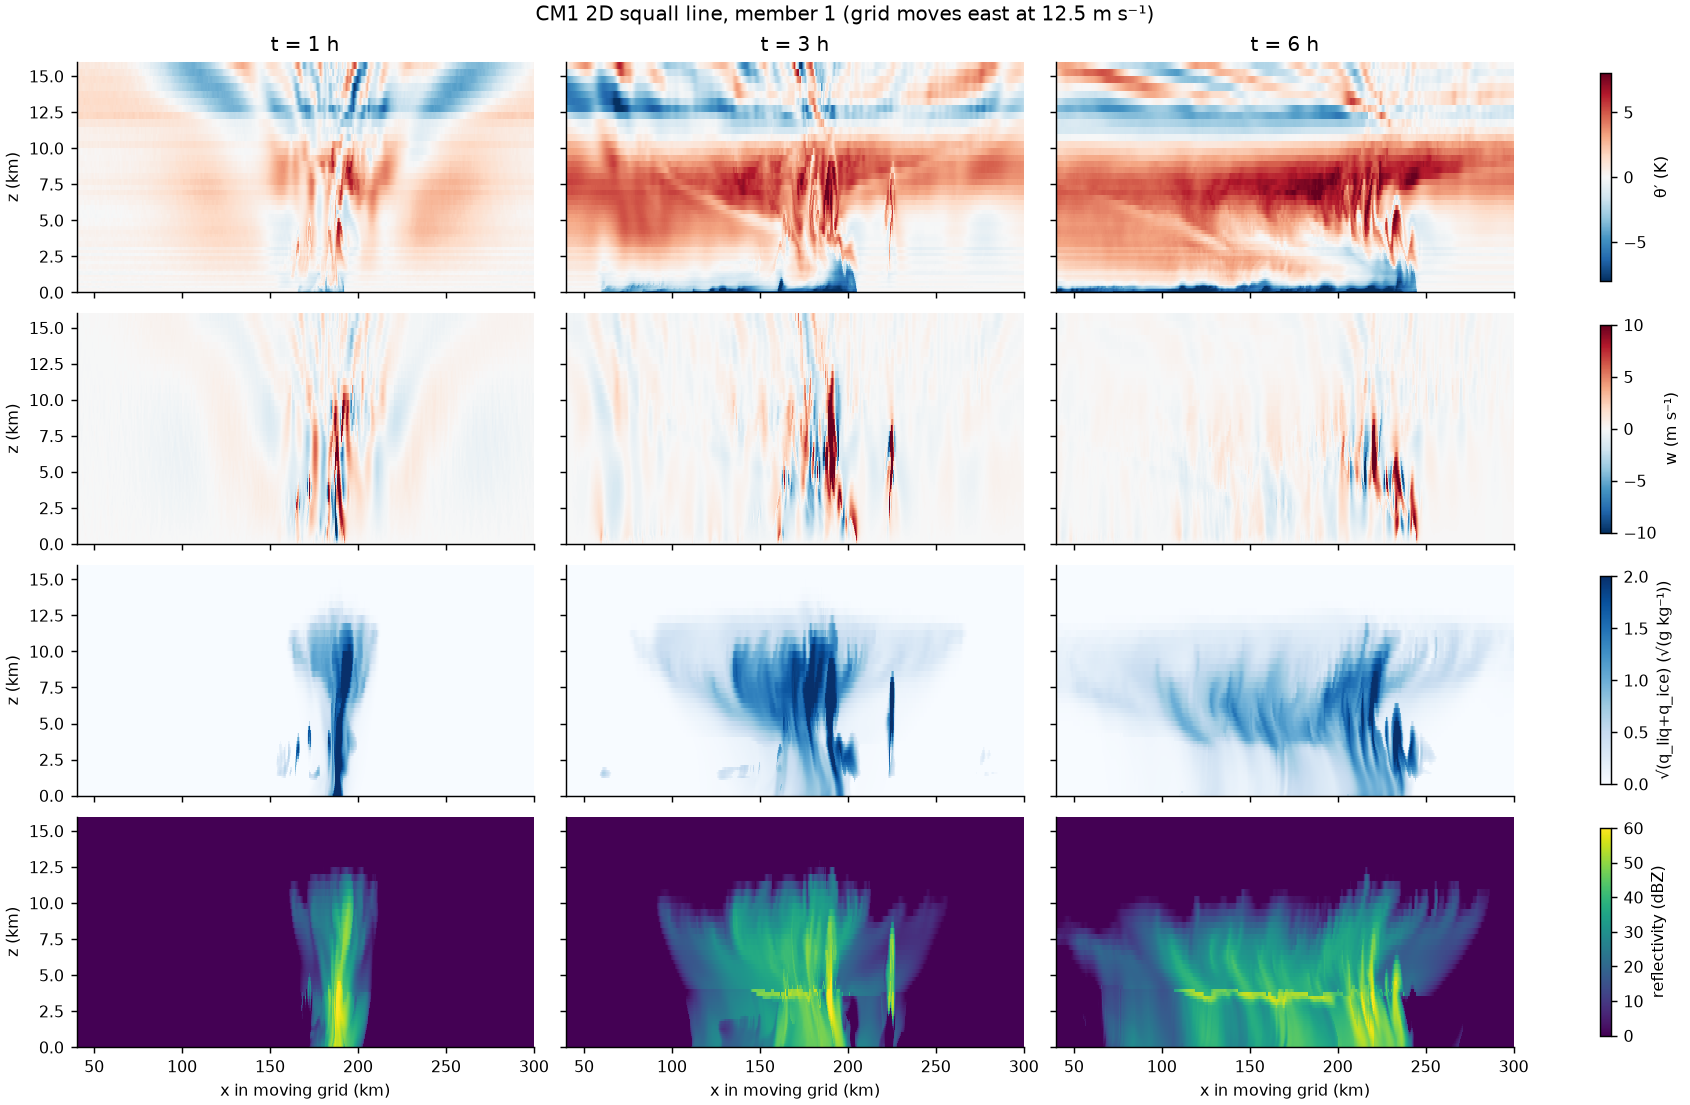
\includegraphics[width=\textwidth]{figs/sections.png}
\caption{Member 1 at 1, 3 and 6\,h. Rows: $\theta'$, $w$, total condensate, reflectivity. Convection starts within 30\,min and a cold pool forms by 1\,h. By 6\,h there is a leading line about 240\,km into the domain, with a stratiform region trailing about 150\,km behind it.}
\label{fig:sections}
\end{figure}

\begin{figure}[h]
\centering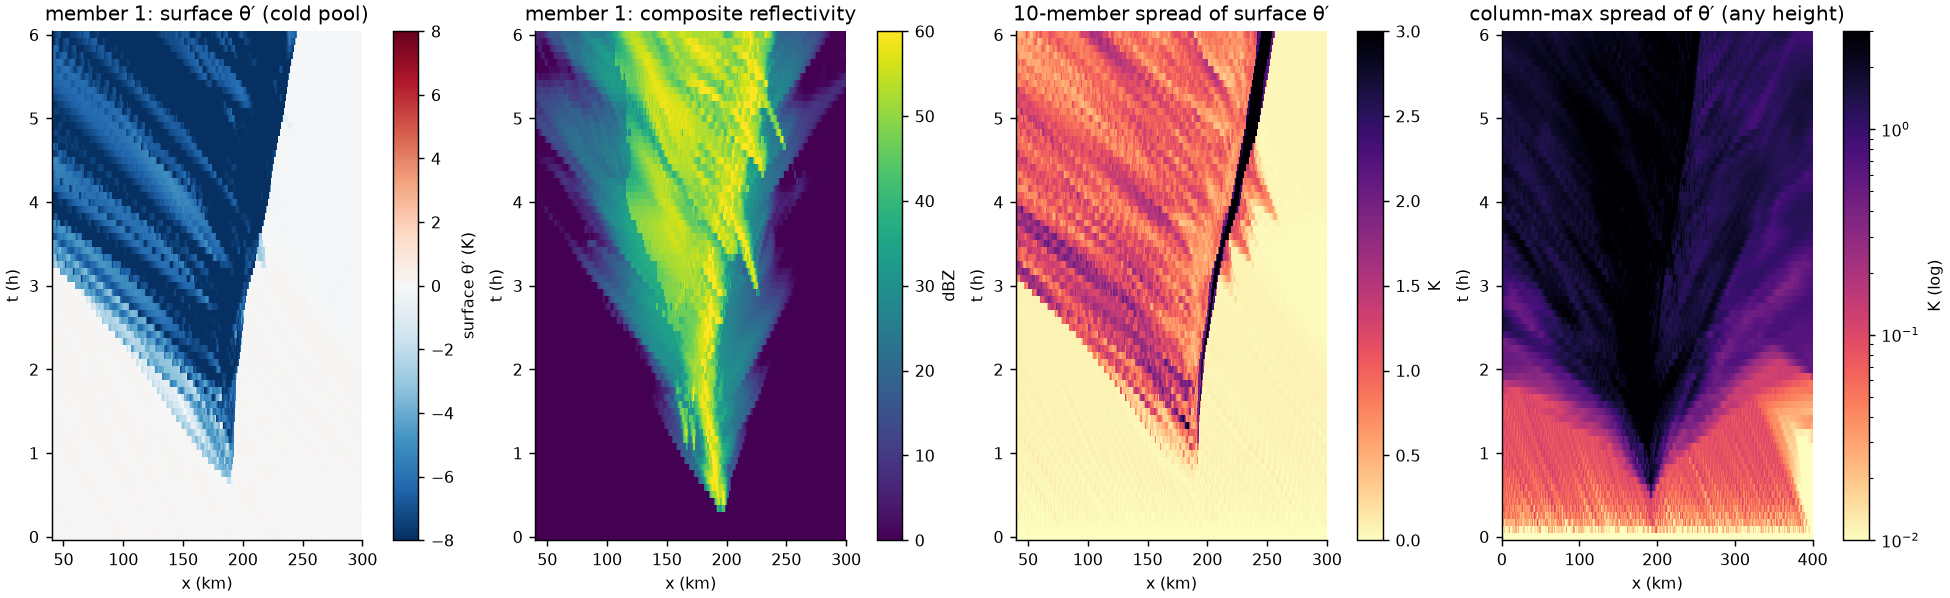
\includegraphics[width=\textwidth]{figs/hovmoller.png}
\caption{Time--distance plots, from left to right: surface $\theta'$ (the cold pool); composite reflectivity; the 10-member spread of surface $\theta'$, which concentrates at the gust front ($>3$\,K), so members differ mostly in front \emph{position}; and the column maximum of the spread (log scale). Regions of member differences above 0.5\,K widen at 19--23\,m\,s$^{-1}$ relative to the grid, faster than the gust front (2.5--3.3\,m\,s$^{-1}$); the likely carrier is gravity waves aloft.}
\label{fig:hov}
\end{figure}

\section{Three questions answered from the data alone}
\paragraph{Is the dynamics local at the output interval?}
We predicted one column 5 minutes ahead from a window of neighbouring columns. Columns were compressed to 32 principal components. The predictors were linear regression and a small neural net; training used members 1--7 and testing used members 9--10. Skill against persistence stops improving at a half-width of 8--12\,km (Figure~\ref{fig:loc}). That agrees with the independent estimate from the spread front in Figure~\ref{fig:hov}, 6--7\,km per frame. With 2\,km sites, this is a stencil of 5--6 sites per 5-minute step, similar to what worked for the Kuramoto--Sivashinsky equation and Kolmogorov flow.

\begin{figure}[h]
\centering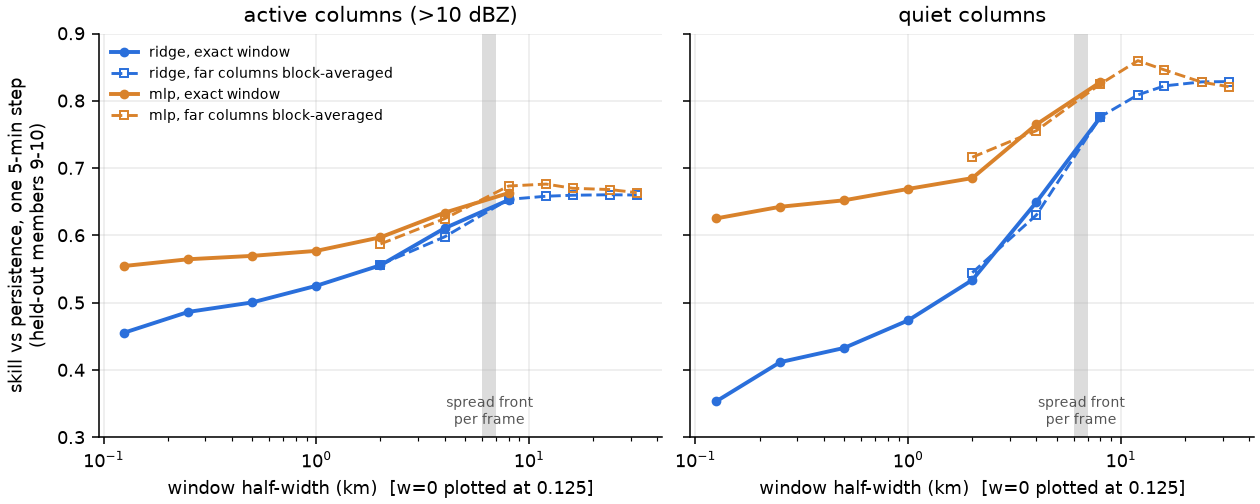
\includegraphics[width=0.85\textwidth]{figs/locality.png}
\caption{One-step skill against window half-width, for storm columns (left) and quiet columns (right). Solid lines use an exact window; dashed lines block-average the far columns. The grey band is the per-frame reach of the spread front from Figure~\ref{fig:hov}.}
\label{fig:loc}
\end{figure}

\paragraph{How much data is needed, and do patches help?}
Cutting patches from the data is valid here. The domain has no terrain and the base state is uniform in $x$, so a patch at any $x$ is a legitimate sample. Patches are not independent storms, though. The 5-minute changes in a column decorrelate within 2 frames and 2--4\,km, but the column states themselves stay correlated for more than an hour and 25\,km.

The learning curve (Figure~\ref{fig:lc}) shows skill rising with the number of training \emph{members}. The linear model saturates at 0.66, while the neural net is still improving. Mirror images are exact solutions here, because without Coriolis the equations are symmetric under $x\to-x$, $u\to-u$. Adding them does not help, because a mirrored storm lives in reversed shear. The number of storms and the variety of environments are separate axes.

\begin{figure}[h]
\centering
\begin{minipage}{0.42\textwidth}\centering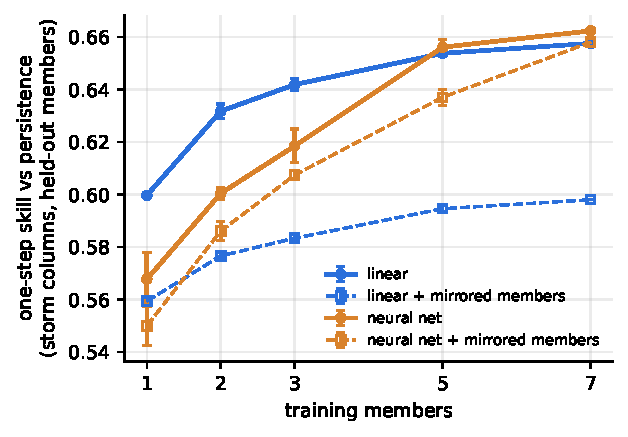
\includegraphics[width=\textwidth]{figs/learning_curve.pdf}\end{minipage}\hfill
\begin{minipage}{0.55\textwidth}
\caption{One-step skill against the number of training members. Three random draws are made per size; error bars are their standard deviation. Training is on members 1--7 and testing on 9--10. The window half-width is 12\,km. The linear model saturates; the neural net is still rising. Mirrored members (dashed) are valid storms in reversed shear, and they do not help predict the original environment.}
\label{fig:lc}
\end{minipage}
\end{figure}

\paragraph{Is 5-minute output fine enough?}
No. We reran member 1's setup for 90 minutes with 1-minute output (Figure~\ref{fig:samp}). The mean squared change of a storm column saturates by a 5-minute interval, and successive 5-minute changes are anticorrelated ($-0.53$). That anticorrelation is the signature of a component that completes a cycle within about two frames; the original 5-minute files show the same ($-0.48$). At 1 minute, successive changes are positively correlated ($+0.37$): the evolution is resolved. This decided the output interval of \texttt{ens\_A}.

\begin{figure}[h]
\centering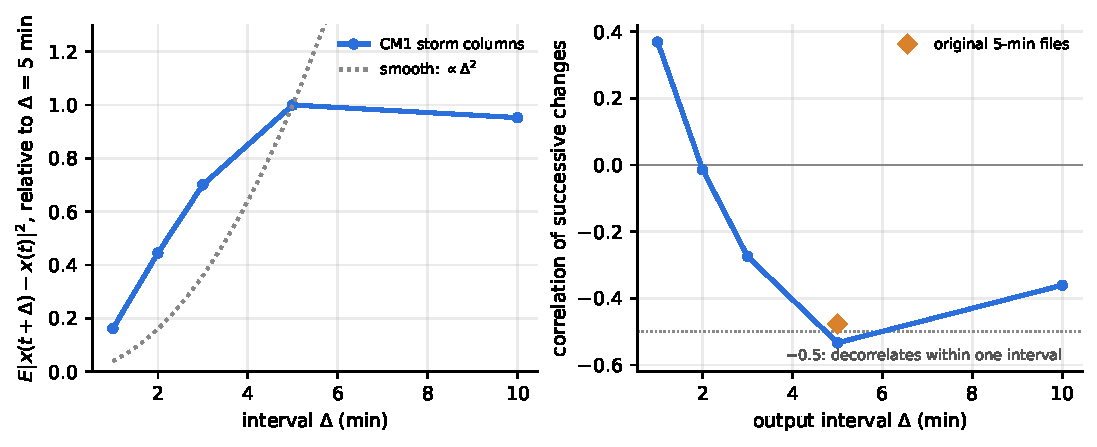
\includegraphics[width=0.85\textwidth]{figs/sampling.pdf}
\caption{Storm columns, 30--90\,min of a 1-minute rerun of member 1's setup. Left: mean squared change against interval, compared with the $\Delta^2$ growth of smooth evolution. Right: correlation of successive changes. The diamond is the same quantity from the original 5-minute files.}
\label{fig:samp}
\end{figure}

\section{A learned model}
The model (\texttt{ks\_latent/cm1}) carries over the design of Papers~I--II, with three changes for CM1:
\begin{itemize}
\item \textbf{Columns as channels.} Locality is horizontal only. Vertical structure and the coupling between variables are learned within each site, which suits a vertically inhomogeneous atmosphere with column-wide pressure coupling.
\item \textbf{Open boundaries.} No periodic padding is used anywhere. In forecasts, the true state is imposed at the domain edges, as for a limited-area model.
\item \textbf{Non-negative condensate.} The decoder output for condensate cannot go below zero.
\end{itemize}
The autoencoder maps each 2\,km site (8 cells $\times$ 434 channels) to 16 latent channels. The propagator is a residual local stencil, exactly the identity at initialization. Its reach per step is set from the measured information speed: 12\,km per 5-minute step, 6\,km per 1-minute step. It is trained with the forced halo of Papers~I--II. Unit tests confirm three properties exactly:
\begin{itemize}
\item shift equivariance in the interior;
\item receptive fields equal to the designed reach;
\item forced-halo window rollouts identical to full-domain rollouts, with a negative control when the halo is too thin.
\end{itemize}

\begin{table}[h]
\centering\small
\begin{tabular}{lccccc}
\toprule
Model & recon.\ $\nmse$ & \multicolumn{3}{c}{forecast $\nmse$ at 5 / 30 / 60 min} & front error, 5--20 min \\
\midrule
5-min, 7 members (Mac) & 0.036 & 0.141 & 0.251 & 0.271 & 0.75--1.2\,km \\
1-min, 28 members, $k\le20$ & 0.030 & \textbf{0.090} & 0.230 & 0.319 & 0.3--0.6\,km \\
1-min, 28 members, $k\le45$ & 0.030 & 0.105 & \textbf{0.217} & \textbf{0.249} & 0.4--0.8\,km \\
\midrule
persistence (1-min test set) & -- & 0.430 & 0.590 & 0.748 & 0.7--3.4\,km \\
truth-member spread & -- & 0.27 & 0.25 & 0.27 & -- \\
\bottomrule
\end{tabular}
\caption{Held-out members. $\nmse$ is the mean squared error over all channels, each variable scaled to unit RMS. Forecasts start from the encoded truth at 1, 2, 3, 4 and 5\,h. The 5-minute model is tested on members 9--10, the 1-minute models on \texttt{mem029}--\texttt{030}. ``Truth-member spread'' is the RMS difference between the two test members divided by $\sqrt2$, roughly the error of a perfect model started from another member.}
\label{tab:fc}
\end{table}

\begin{figure}[h]
\centering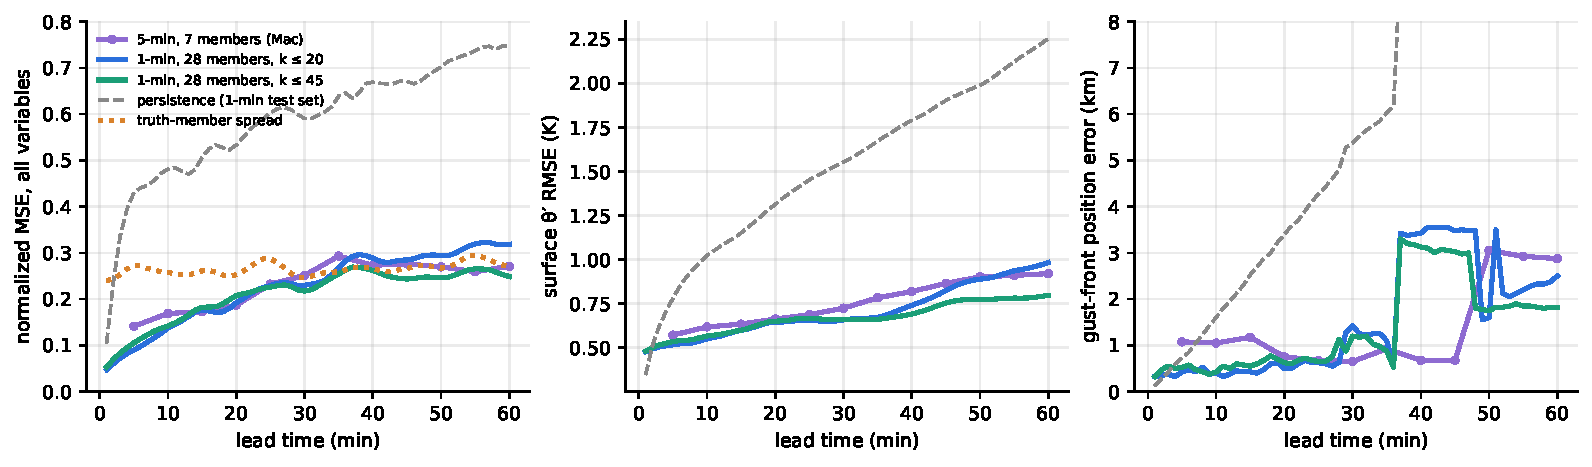
\includegraphics[width=\textwidth]{figs/forecast_comparison.pdf}
\caption{Forecast error against lead time for the three models in Table~\ref{tab:fc}. One-minute output with four times the members cuts the 5-minute error by 36\%. Training on longer rollouts ($k\le45$) keeps the error below the truth-member spread for the whole hour, at a cost of 10--15\% at 1--5 minutes.}
\label{fig:fc}
\end{figure}

\begin{figure}[h]
\centering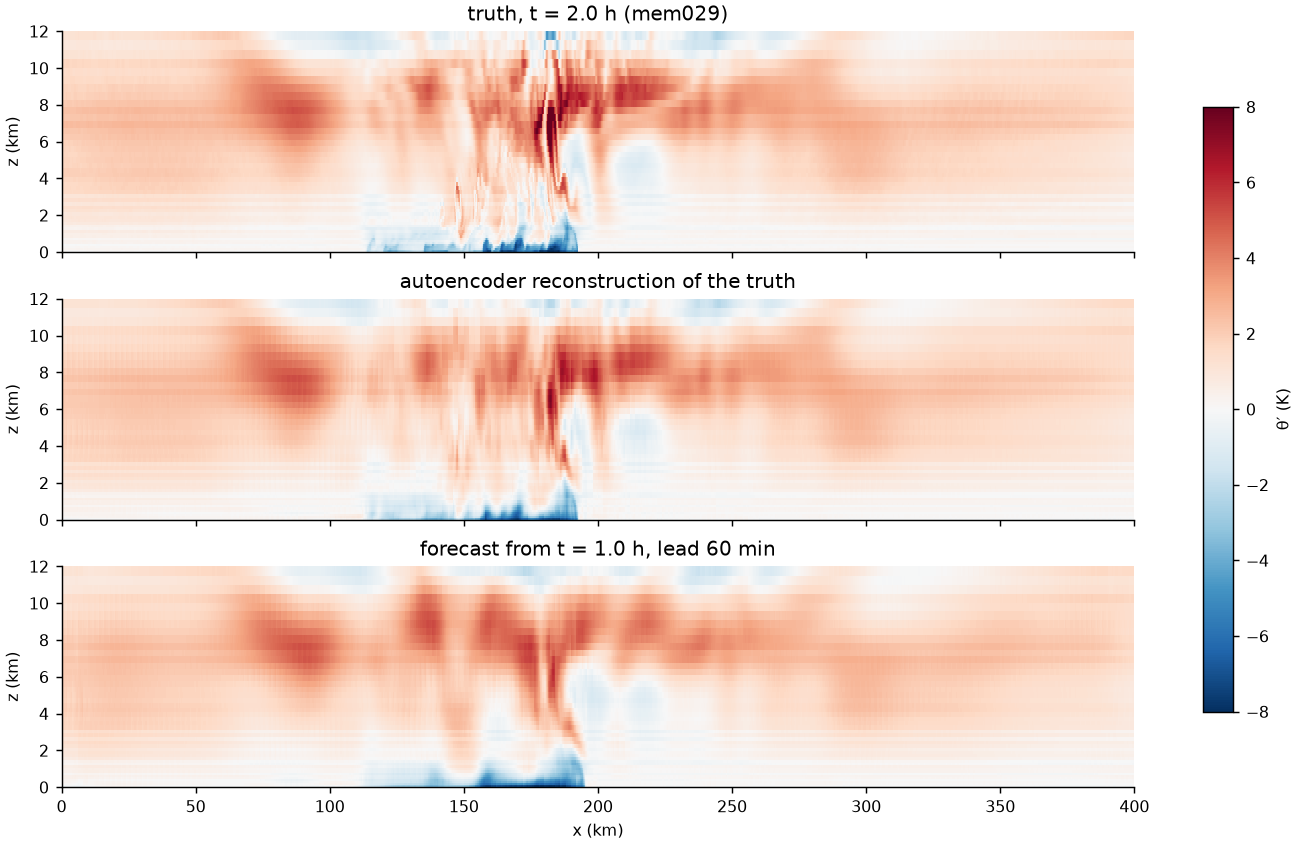
\includegraphics[width=\textwidth]{figs/forecast_sections_k45.png}
\caption{Potential temperature perturbation for test member \texttt{mem029} at 2\,h: the truth, the autoencoder reconstruction, and the 60-minute forecast from 1\,h ($k\le45$ model). The forecast keeps the cold pool, the front near $x=190$\,km and the main warm plume aloft, and smooths the small convective cells.}
\label{fig:fcsec}
\end{figure}

Three conclusions so far:
\begin{itemize}
\item \textbf{The 5-minute model is at the limit of its data.} Its one-step skill against persistence (0.67) equals the model-free ceiling of Figure~\ref{fig:loc}. Doubling the latent channels improves reconstruction but not forecasts.
\item \textbf{Finer time sampling and more members both help.} With 1-minute frames and 28 members, the 5-minute skill rises to 0.79.
\item \textbf{The remaining long-lead error came from the training horizon,} and longer training rollouts remove most of it.
\end{itemize}

\FloatBarrier
\section{Open questions and next steps}
The task list is in \texttt{docs/cm1\_plan.md}. The main questions are:
\begin{enumerate}
\item Does skill keep rising with more storms at 1-minute output (a learning curve with 56 members)?
\item Does the model generalize to environments it has not seen, such as other low-level moisture and shear?
\item Does it respect the physics, e.g.\ mass divergence of decoded states and condensate budgets?
\item The data-assimilation question of Paper~III: with a per-site latent filter, open boundaries, surface $\theta'$ and nonlinear reflectivity observations, does it track a held-out storm better than the free model?
\end{enumerate}
\end{document}
